\documentclass[12pt,a4paper,final]{article}
\usepackage[latin1]{inputenc}
\usepackage{amsmath}
\usepackage{amsfonts}
\usepackage{amssymb}
\usepackage{graphicx}


\usepackage[english]{babel}
\usepackage[latin1]{inputenc}
%\usepackage[leqno]{amsmath}

\usepackage{textcomp}
\usepackage{mathrsfs,euscript}
\usepackage{booktabs}
\usepackage{dcolumn}
\usepackage{epsfig}
\usepackage{upref}
\usepackage{paralist}
\usepackage{calc}
\usepackage{setspace}
%\usepackage[parfill]{parskip}
\usepackage[left=3.5cm,right=3.5cm,top=2cm,bottom=2cm]{geometry}
\usepackage[longnamesfirst]{natbib}
\bibliographystyle{plainnat}
%\usepackage{biblist}
%\usepackage{chicago}
%\bibliographystyle{chicago}
\usepackage{graphicx,float}
\usepackage{graphics}
\usepackage{multicol}
\usepackage{float}
\usepackage[normalem]{ulem}
\author{Eliab G. Luvanda}

\title{Construction of Business Cycle Indicators \\
\textit{REPORT} \\
Submitted to \\
\textbf{Tanzania Revenue Authority (TRA)}}

\date{March 7, 2016}
\begin{document}

\maketitle

\newpage
\tableofcontents

\listoffigures

\listoftables

\newpage
\section{Introduction}

\subsection{Background}
Business cycles are output fluctuations that involve movements in GDP overtime in alternating periods of expansion in economic activity (boom) and contraction in economic activity (recession). GDP/output being a base of tax revenue, business cycles are usually associated with fluctuations in tax revenue.  The upwardand downward swings in macroeconomic variables include GDP growth of domestic  and external economies, inflation, exchange rate, credit to the private sector, investment levels and more others.  These variables need to be monitored to detect their short and medium term influence on revenue collection. This study estimates business cycles and  examines how the cycles influence tax revenue, and more specifically to what extent business cycles influence flucuations in tax revenue in Tanzania.  

Business cycles in this case means fluctuation in output/GDP, which is the overall tax base, and also fluctuations in sectoral output/GDP, constituting bases for different taxes. In this case, tax revenue is defined in a way that excludes non-tax revenue.  Regarding tax revenue, this study covers tax revenue from the major sectors: agriculture, industry and services. In terms of time coverage, the period from 1966 to 1994 has been covered by the study for the estimation of business cycles. The reason for this is that a reasonable long time coverage is needed for obtainint reliable estimates of business cycles.  Given the fact that the main  tax categories for which the data is avalable for the entire 1966-2014 period are income tax, import and excise duties, and others (as a tax category), business cycles have been estimated for only those broad tax categories. 

\subsection{Objective of the assignment}
In view of the fact that business cycles have a significant impact on tax revenue, this study estimates business cycles and examines how they are related  to revenue collection performance.  That is the main objective of this study.  The specific objectives include the following:

\begin{compactenum}[1)]
\item Examine the nature, main features and causes of business cycles in Tanzania and the associated reasons for their occurrence. Two (2) main tasks will have to be undertaken to address this specific objective. The first task will be to estimate and examine the trends and cyclic components of output (GDP), and other macroeconomic variables such as private consumption, investment, money stock, government expenditure, tax revenue, and the general price level/consumer price index (CPI) and the main characteristics of business cycles in Tanzania.  Specifically, the following two issues will have to be addressed; namely:
\begin{compactenum}[(i)]

\item	Using the relevant time series filters such as the Hodrick-Prescott (HP) filter, and Baxter-King (BK) filter to estimate the trend/permanent and cyclic components of macroeconomic variables (including GDP, sectoral GDP, private consumption, government expenditure, imports, inflation, exchange rate and tax revenue); and examining their patterns, such as the volatility of fluctuations/cyclic components;

\item b)	Identifying macroeconomic variables that are pro-cyclic (move together with output/GDP), and macroeconomic variables that are counter-cyclic (move in different directions with output/GDP) over the business cycle.
\end{compactenum}  

\item	Analyze economic sectors' behavior and  sectoral revenue data and determine the more responsive sectors in terms of upward and downward movements as well as their impact on revenue. This objective requires examining the behavior of economic sectors (such as agriculture, manufacturing, services, mining etc); and examine how the sectoral performance influence tax revenue.  More specifically, this objective will require the study to carry out the following:

\begin{compactenum}[(i)]
\item	Examine the sectoral performance (in terms of output) trends, and relative contribution of sectors to GDP;

\item	Examine the sectoral performance over the business cycle.  This will involve decomposing sectoral output into trend and cyclic components and examine the patterns of the components over time.  In addition the study will have to measure the volatility of sectoral output fluctuations over over the business cycle. 

\item Examine the extent to which tax revenue responds to movements in sectoral output in 2)(i) and 2) (ii) above. 

\end{compactenum}

\item 	Examine the extent to which tax revenue responds to both long term and cyclic movements of GDP/output. This will involve the following:

\begin{compactenum}[(i)]
\item	Examining how tax revenue responds to long-term movements in GDP and sectoral output/GDP. Basically, this will involve carrying out cointegration test to examine whether there is a long run equilbrium relation ship between output and tax revenue.

\item Examining how tax revenue responds to short-term movements in GDP and sectoral output/GDP.  
\end{compactenum}

\item Prepare a model report on Tanzania business cycles linking with tax collection.  This will involve coming up with a report, which among other things, will include a model linking tax revenue with business cycles.
 
\end{compactenum}




\section{Methodology}
The specific objectives of the study have guided the design of the  methodology. This section explains the study methododology  and how the different aspects of the methodology do address the specific objectives of the study.

\subsection{Literature Review}

Both theoretical and empirical literature related to business cycles and the behaviour of tax revenue over the business cycle have been reviewed.  The main aim of this review was to explore the theory behind business cycles in relation to tax revenue and guide the choice of analytical techniques for carrying out the assignment.

\subsection{Data Collection}

Secondary data has been used. Time series data for macroeconomic variables (including tax revenue) has been obtained from official publications (database kept) by the Bank of Tanzania (BOT), the National Bureau of Statistics (NBS), and Tanzania Revenue Authority (TRA).  The International Financial Statistics (IFS) was another source of time series data for the variables.  Qualitative information has been obtained from the publications.

\subsection{Data Analysis}

Data analysis will be carried out to estimate the trend and cyclic components of GDP/output other macroeconomic variables such as tax revenue, inflation, government expenditure and money supply. Data analysis will also involve computation of correlation coefficients, cointegration test and estimation of econometric models to examine the relationsip between output and tax revenue.

\subsubsection{Estimation of Trend and Cylic Components of Macroeconomic Variables}

Standard filters such as the Hodrick ? Prescott (HP) and Baxter King (BK) filters are commonly used to estimate the trend and cyclic components of the variables.  This study will use the Hodrick - Prescott filter, the most commonly used filter in the business cycle studies.

\subsubsection*{Decomposition of Time Series into Trend and Cyclical Components}

A macroeconomic time series   is composed of two main components: (1) the permanent (or secular) component $y_t^p$ , and (2) the transitory component  $y_t^c$. Thus, a macroeconomic variable can be represented by the following simple model:

\[ y_t = y_t^p + y_t^c \]

where $y_t$  is logarithm of actual observation, $y_t^p$  is a trend or secular component and $y_t^c$  represents deviations from trend or a cyclical component.  Stochastic detrending methods can be used to estimate the trend and cyclic components of macroeconomic variables. The most popular among the stochastic detrending methods is the Hodrick Prescott  (hereafter referred to as HP) (1980) filter.  The other and more recent is the Baxter--King (1995) filter. The HP trend for a variable $y_t$ (in logarithmic form) is found by minimizing the following function:

\[ \sum_{t=1}^T\left( y_t - y_t^{trend}\right) ^2 + \lambda \sum_{t=2}^{T-1} \left[ \left( y_{t+1}^{trend} - y_t^{trend}\right) -\left( y_t^{trend} - y_{t-1}^{trend}\right)  \right] \]

The idea behind this equation is to minimize the sum of two components.  The first component is the sum of squares of the deviation of the actual value of a variable from its trend value.  The second is the sum of squares of changes in the trend growth.  A series of trend values that gives the minimum value of the equation is the HP trend or filter.
A parameter, $\lambda$, controls the degree of smoothness in the HP trend.  On the one hand, a smaller value of $\lambda$ reduces the importance of change in trend growth.  For $\lambda = 0$, a minimum value of the equation is given by selecting the trend value equal to the actual value of the variable.  In this case, there cannot be deviations from trend.  On the other hand, a very high $\lambda$ diminishes the significance of the first component.  In the limit, a smooth deterministic trend yields the minimum of the total sum, and the cyclical component of a variable will be large. 

To get a `reasonable' variable trend, one must choose an intermediate value of $\lambda$.  Hodrick and Prescott (1980) recommend $\lambda = 1600$ for quarterly data, and $\lambda = 100$ for annual data.  However, Ravn et al (1997) recommend $\lambda = 6.75$ for annual data. Once a trend component, has been estimated, the cyclical component of the variable can be obtained by subtracting the trend value from the actual observations of the variable; that is, $y_t^c = y_t - y_t^p$. 

Once the trend and cyclic components have been estimated, they are usually plotted on a graph from which one can study the pattern of long term movement of the variable, and the pattern of cyclic movement/fluctuations of the variable.

Preliminary estimates of cyclic and trend components for some of the macroeconomic variables are attached as an Appendix.

\subsubsection{Computation of Correlation Coefficients and Variances}

Once the cyclic components of the variables have been estimated, as explained in the preceding section, correlation coefficients between the cyclic component of output/GDP (as a reference variable) and cyclic components of other macroeconomic variables (including tax revenue).  The correlation coefficients (negative or positive) will help in determining whether the other macroeconomic variables are are procyclical (the cyclic component of the variable move in the same direction as the cyclic component of output/GDP); or whether the other macroeconomic variables are counter-cyclical (the cyclic component of the variable move in the different relative to the cyclic component of output/GDP). Variances of the cyclical components of the variables will be computed to measure the volatitilty of fluctuations of the economic variables over the business cycle.

\subsection{Econometric Analysis}

Econometric analysis will be employed to examine the main factors (monetary and real factors) that drive the busines cycles in Tanzania; and to examine long term movements in output do influence tax revenue (categories of tax revenue), and whether short term movements over the business cycle in output do influence tax revenue.

\subsubsection{Vector Autoregression (VAR) Model} 

A simple vector autoregression (VAR) model will be estimated and used to examine the relative importance of monetary and real factors in explaining the variations in output. The following VAR model will be estimated:

\[ Y_t = \Phi_0 +\Phi_1 Y_{t-1} + \ldots + \Phi_p Y_{t-p} + \varepsilon_t \]

where $Y_t$ is a vector of output, monetary and real factors, $\Phi_0$ is a vector of constants, $\Phi_i$ ($i=1,\ldots,p$) are coefficient matrices; and $\varepsilon_t$ is a vector of error terms that are assumed to be independent and identically distributed.

Once the VAR model has been estimated, ganger causality test will be used to examine whether monetary or real factors do influence output. The variance decompostion will be used to examine the relative importance monetary and real factors in explaining the business cycles.

\subsubsection{Cointegration Test}

Cointegration test will be carried out to examine whether there is a long run equilibrium relationship between GDP/output/sectoral GDP and tax revenue/categories of tax revenue. In other words this test will help in determining whether tax revenue respond to long term movement in output/GDP. The output/GDP coefficient in the cointegrating equation will be the measure of long run tax elasticity

\subsubsection{Estimation of Simple Econometric Models}

Simple econometric models will be estimated to examine how tax revenue responds to short run movements in output/GDP over the business cycle. The following simple model will be estimated:

\[ T_t^c = \alpha + \beta Y_t^c + \varepsilon_t \]

where $T_t^c$ is cyclical component of cyclic tax revenue, and $Y_t^c$ is cyclic component of output/GDP. In this case, cyclic components of different tax revenue will be estimated as a function of cyclic component of the tax base.

\subsection{Software package}
\textbf{R}, an open source programming environment,  will be used for data analysis. 

\section{Main Findings of the Study}

\subsection{Sectoral Perfomance Trends}

In this section, the peformance of the major sectors is examined.  More specically, the section analyses the trends of contribution of the sectors to GDP and tax revenue over time.  The section also examines the growth patterns in terms of both output and revenue generation.

\newpage
\subsubsection{Contribution of Sectors to GDP}

The services sector contributes the largest share to GDP.  It's share is about 48 percent.  The share has been rising slightly overtime; from 46 percent in 1998 to 48 percent in 2013 (See Figure 1 below). Agriculture is the next important sector in terms of contribution to overall GDP.  Its share in total GDP is about 27 percent.  However, the relative importance of this sector to GDP contribution has been decreasing gradually; from 32 percent in 1998 to 27 percent in 2013.
\begin{figure}[hbt]
\centering
\begin{small}
\caption{Trends of Sectoral Shares in GDP}
\end{small}
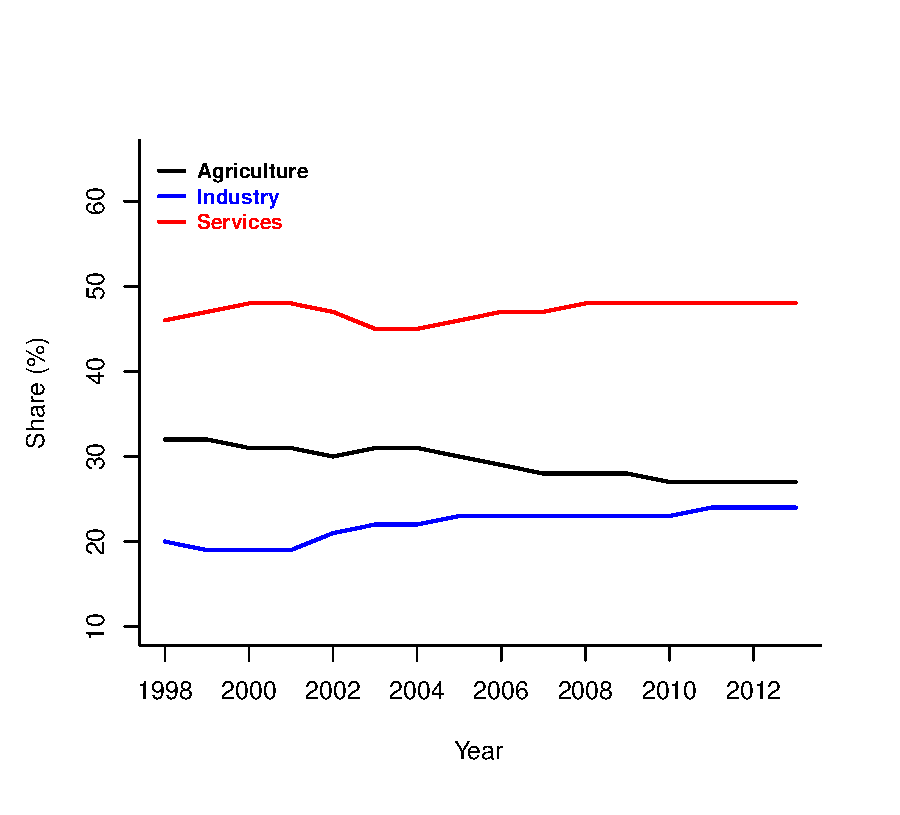
\includegraphics[scale=0.501]{shares.eps} 
\end{figure}

Industry contributes the smallest share; in the sense that it contributes about 24 percent.  However, the share of this sector has been gradually increasing; from about 20 percent in 1998 to about 24 percent in 2013.


\subsubsection{Contribution of Sectors to Tax Revenue}

Just like in the case of contribution by sectors to GDP, the services sector contributes the largest share to tax revenue.  Its share is about 69.8 percent. 

\begin{figure}[hbt]
\centering
\begin{small}
\caption{Trends of Sectoral Shares in Tax Revenue (\%)}
\end{small}
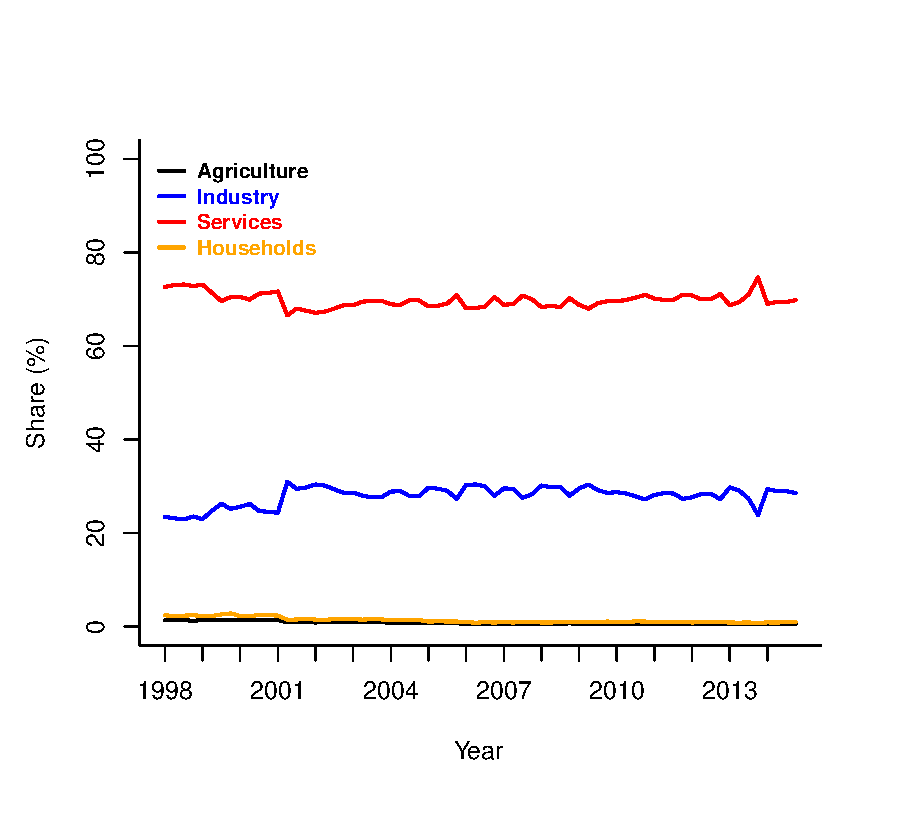
\includegraphics[scale=0.501]{rev_sec_shares.eps} 
\end{figure}

This share has more or less being constant over a decade. Next in importance, but trailing behind by far is the industry sector which, on evarage, contributes about 28.5 percent to tax revenue. The contribution of the agriculture sector to tax revenue is almost neglible, about 0.8 percent.  Households' contribution to tax revenue is about 1.4 percent.

Table 3 below presents trends of revenue generation by sectors. However, it should be noted that because of large differencs in absolute figures of the sectors, the logarithm scale on the vertical axis has to be used for the convenience of comparison.

\begin{figure}[ht]
\centering
\begin{small}
\caption{Trends of Tax Revenue by Sectors}
\end{small}
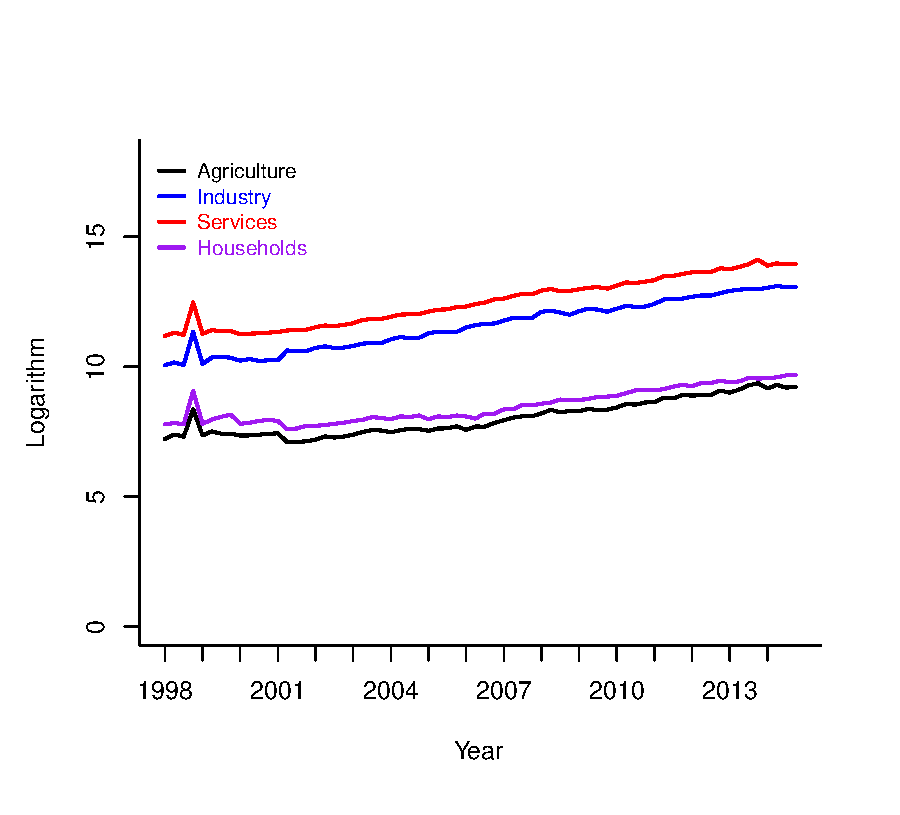
\includegraphics[scale=0.501]{rev_sec_trends.eps} 
\end{figure}

As the Figure shows, generally speaking, tax revenue from all sectors increased over time.  However, estimates of revenue growth for the 1998-2013 period suggest that tax revenue from the industry sectry sector relatively rose at the highest rate of 4.8 percent, followed by the services sector at 4.6 percent. \footnote{Estimates of growth rates are presented in Table 3 in the Appendix}  Low growth rates characterised the agriculture and household sectors, with the growth rates of 3.2 percent and 3 percent, respectively.

\subsection{Business Cycles}

This Subsection presents estimates of business cycles. A standard Hodrick-Prescott filter has been used to decompose the macroeconomic variables: GDP, inflation,  money supply - broadly defined (M2), government expenditure and tax revenue into trend and cyclic components. As it has been mentioned in the methodology Section, business cycles for the three broad categories of tax revenue: (1) income tax, (2) import and excise duties, and (3) other taxes have been estimated because the data covering the 1966 - 2013 period is available only for these broad categories, rather than for the more disaggregated categories of tax revenue.

\subsubsection{GDP}

Figure 4 below presents the thrend and cyclic components of real GDP. A closer examination of the Figure reveals that Tanzania experienced 3 main cycles between 1966 and 1992, and mild economic fluctuations therefater. 

\begin{figure}[ht]
\centering
\begin{small}
\caption{Trends and Cyclic Components of Real GDP}
\end{small}
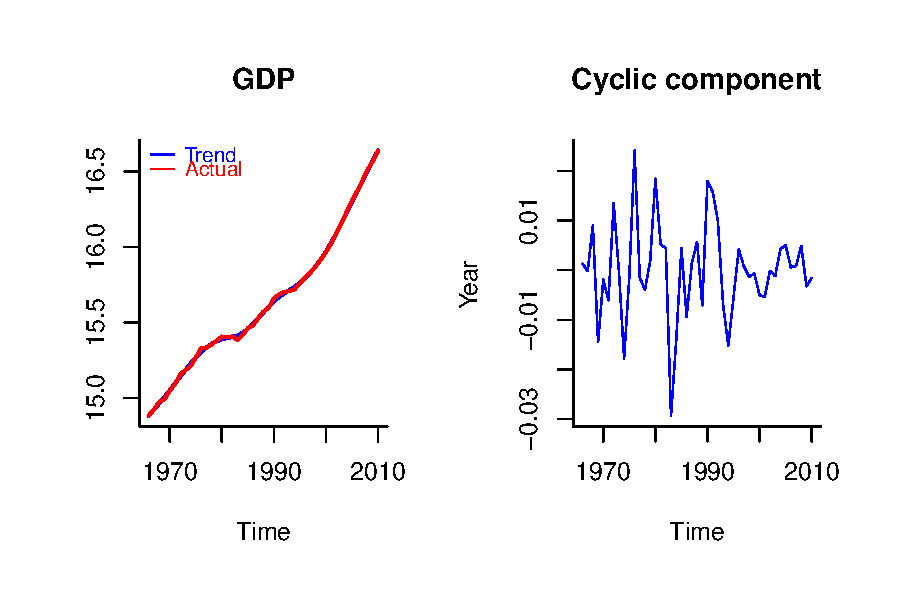
\includegraphics[scale=0.601]{gap_comp.eps} 
\end{figure}

The first major business cycle over the study period occured from 1966 to 1972.  This cycle took 6 years.  The second major cycle occured between 1972 and 1976, and it lasted for approximately 4 years. The last major business cycle, and actually the longest one occured between 1976 and 1992, and it lasted for approximately 16 years. The deviation of actual GDP from trend was at its peak in 1972, when the economy recorded a 6.5 percent growth rate. A deep recession occured in 1983, when the economy recorded a negative growth rate of 2.4 percent, the lowest growth rate ever in the post-independence Tanzania's history.

\subsubsection{Money Supply - Broadly Defined (M2)}

Figure 5 presents an estimate of the cyclic component of money supply - broadly defined (M2). On the right panel of the Figure a cyclic component of GDP is presented for comparison.

\begin{figure}[ht]
\centering
\begin{small}
\caption{Cyclic Component of Money Supply}
\end{small}
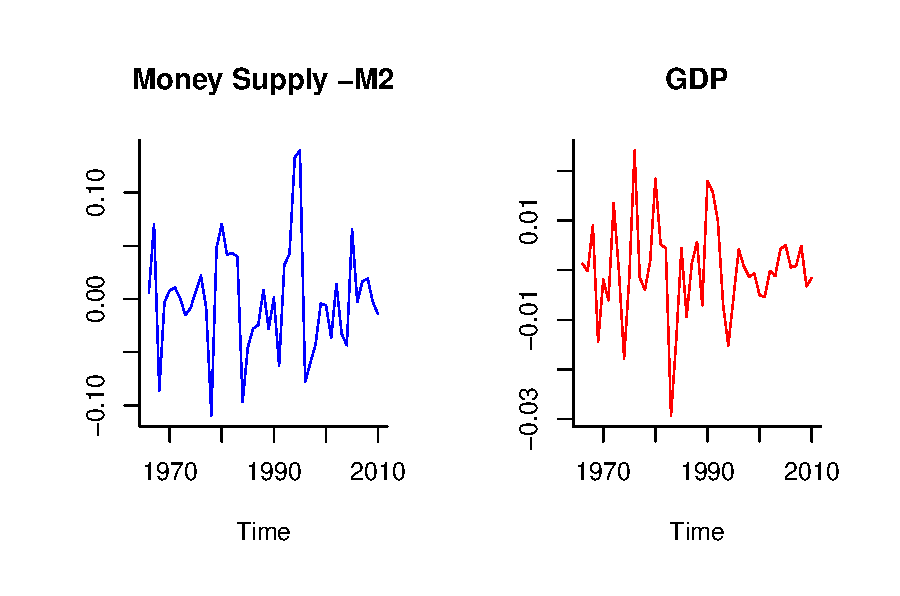
\includegraphics[scale=0.601]{money_supply.eps} 
\end{figure}

Just like in the case of GDP, money suply is characterized by 3 business cycles between 1966 and 1995, and relatively milder fluctuations thereafter. Somehow, this could be a reflection of the government's commitment to a stable monetary policy in the post economic reform period. 

\subsubsection{Inflation}

The estimate of cyclic component of inflation is presented in Figure 6, and on the right panel of the Figure is the estimate of the cyclic component of GDP for comparison. As it has been noted in the case of GDP and money supply, the cyclic component of inflation is charactrized by big fluctuations between 1966 and 1992, and milder fluctuations after 1992. 

\begin{figure}[ht]
\centering
\begin{small}
\caption{Cyclic Component of Inflation}
\end{small}
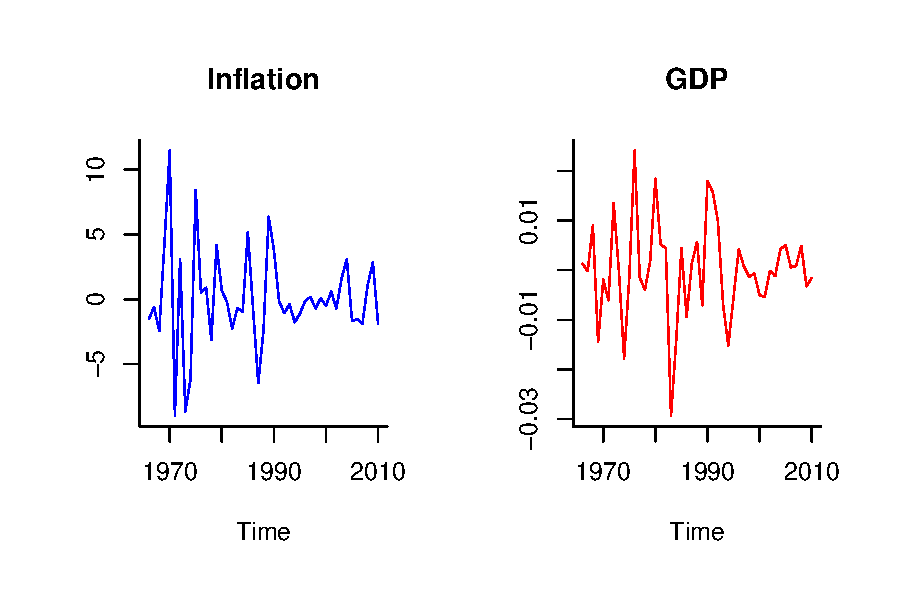
\includegraphics[scale=0.601]{inflation.eps} 
\end{figure}

When the cyclic components of money supply and inflation it appears that the cyclic component of inflation is characterized by a higher frequency of fluctuations than that of money supply. This in a way, suggest that inflation in Tanzania is not purely a monetary phenomenon; and that other real and structural factors influence the rate of inflation.

\subsubsection{Government Expenditure}

Figure 7 presents the estimate of the cyclic component of government expenditure, and also an estimate of the cyclic component of GDP for comparison.

\begin{figure}[ht]
\centering
\begin{small}
\caption{Cyclic Component of Government Expenditure}
\end{small}
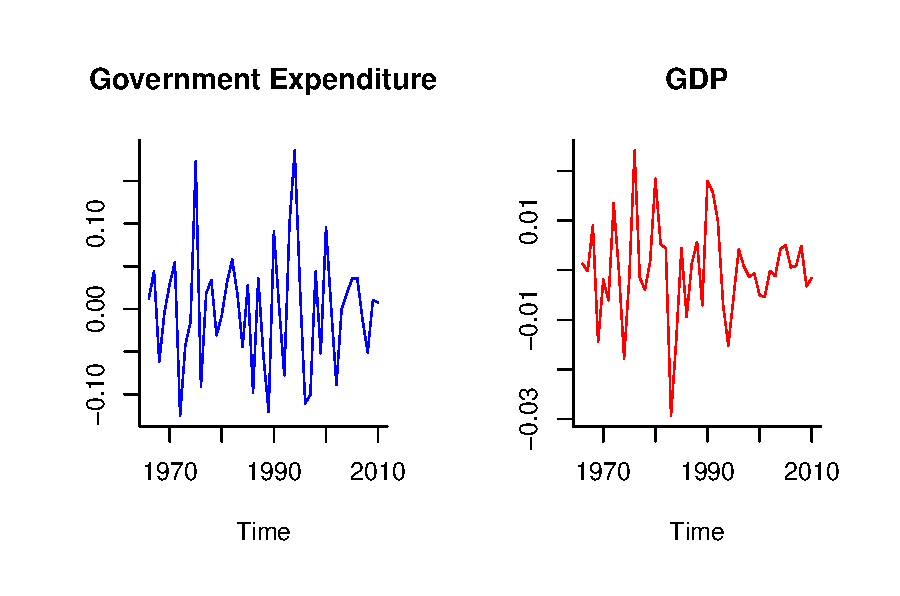
\includegraphics[scale=0.601]{gov_expend.eps} 
\end{figure}

More or less the cyclic component of government expenditure behaves like those of GDP, money supply, and inflation.  It is characterised by big fluctuations between 1996 and 1992, and relatively milder fluctuations after 1992. This in a way could be reflecting the government's commitment to a more stable fiscal policy in the post economic reform period.

\newpage
\subsection{Business Cycles and Tax Revenue}

In this section, estimates of business cycles for tax revenue are presented.  Cyclic components of total tax revenue, income tax, import and excise duties, and othe taxes (as a category) have been estimated for the period 1966 - 2013. It was not possible to estimate the cyclic components of more disaggregaed categories of taxes due to unavailability of data before 1998. In addition to presenting the esstimates of the cyclic componts of the tax revenue, the behaviour of these cyclic components is compared to the behaviour of the cyclic component of GDP.

\subsubsection{Total Tax Revenue}

The estimate of the cyclic component of total tax revenue is presented in Figure 8 (left panel). On the right panel, the estimate of the cyclic component of GDP (the major tax base) is presented for comparison.

\begin{figure}[ht]
\centering
\begin{small}
\caption{Cyclic Component of Tax Revnue}
\end{small}
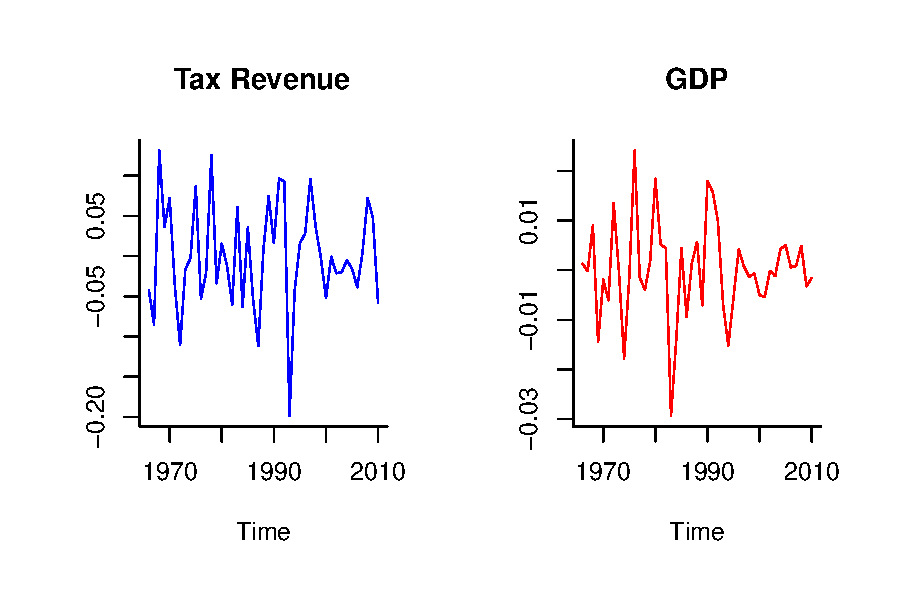
\includegraphics[scale=0.601]{tax_revenue.eps} 
\end{figure}

As it can be observed in the Figure, generally speaking, the cyclic component of total tax revenue behaves more or less like that of GDP.  First, just like in the case of GDP, the cyclic component of total tax revenue is characterized by 3 major cycles between 1966 and 1992, and relatively milder fluctuations thereafter. Second, the peaks and troughs of the two cyclic components are more or less synchronized. For example, both cyclic components are characterized by peaks roughly in 1967, 1976 and 1996.  Similarly, both components are charecterized by troughs roughly in 1970, 1983 and 1992.

\newpage
\subsubsection{Income Tax}

Figure 9 presents the estimate of the cyclic component of income tax together with the estimate of the cyclic component of GDP for comparison.

\begin{figure}[ht]
\centering
\begin{small}
\caption{Cyclic Component of Income Tax}
\end{small}
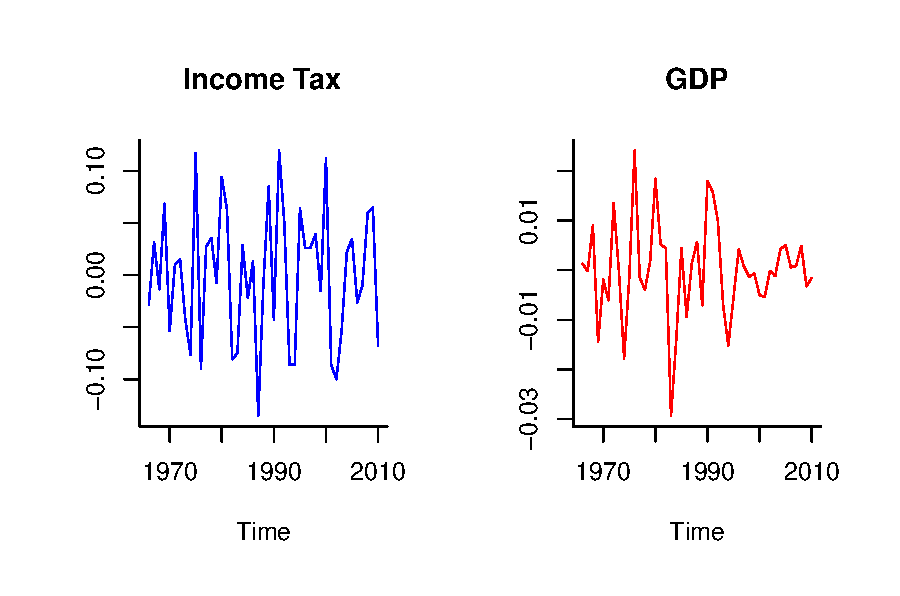
\includegraphics[scale=0.601]{income_tax.eps} 
\end{figure}

A closer observation of Figure 9 reveals that the cyclic component of income tax behave more less like that of total tax revenue.  This is not suprising because income tax is one of the components that make up the total tax revenue. Just like the cyclic component of total tax revenue, the cyclic component of income tax is characterized by 3 major cycles between 1966 and 1992, and a period of relatively mild fluctuations thereafter. The peaks and troughs of the cyclic component of income tax are sychronized with those of the cyclic component of GDP.

\subsubsection{Import and Excise Duties}

The estimate of the cyclic component of import and excise duties is presented in Figure 10. On the right panel of the same Figure, the cyclic component of GDP is also presented for comparison.

\begin{figure}[ht]
\centering
\begin{small}
\caption{Cyclic Component of Import and Excise Duties}
\end{small}
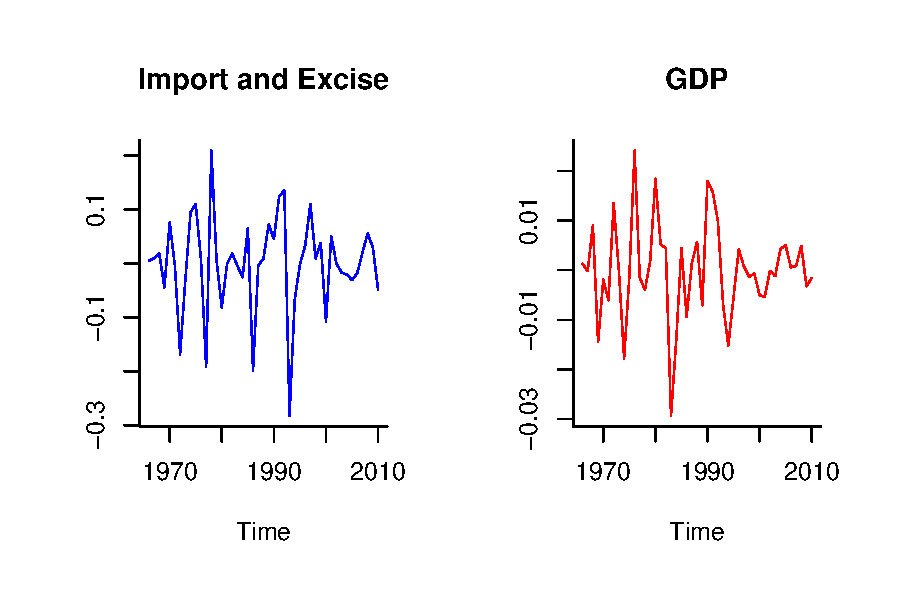
\includegraphics[scale=0.601]{import_taxes.eps} 
\end{figure}

The behavior of the cyclic component of import and excise duties is similar to those of total tax revenue, income tax and GDP. It is also characterized with 3 major cycles between 1966 and 1992, with the period after 1992 being characterized by relatively milder fluctuations.  The peaks and troughs of the cyclic component of import and excise duties are also more or less synchronized with those of GDP.

\subsubsection{Other Taxes}

Figure 11 presents the estimate of the cyclic component of other taxes. In the same Figure, the estimate of the cyclic component of GDP is also presented for comparison.

\begin{figure}[ht]
\centering
\begin{small}
\caption{Cyclic Component of Other Taxes}
\end{small}
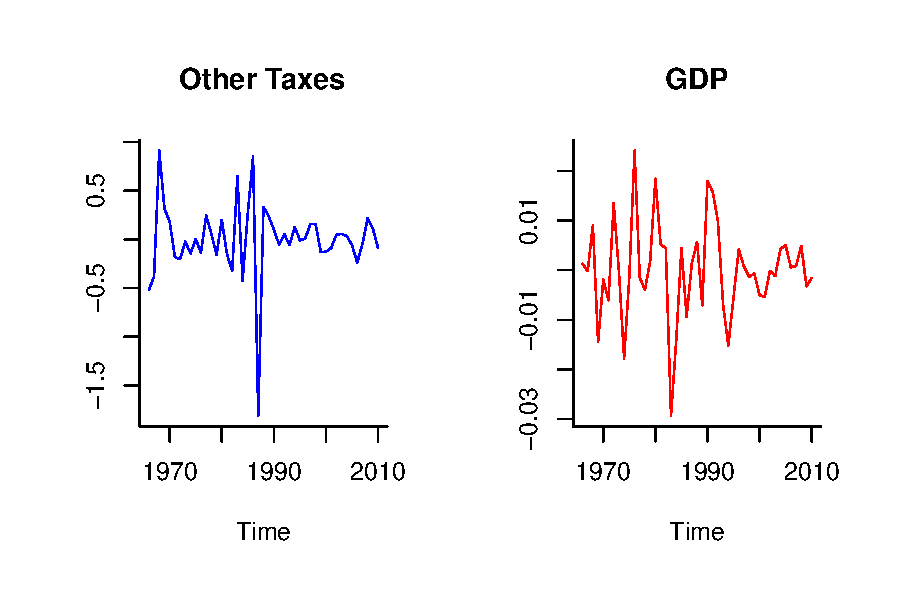
\includegraphics[scale=0.601]{other_taxes.eps} 
\end{figure}

It is interesting to note that the cyclic component of other taxes behave significantly differently from the cyclic components of GDP and those of other macroeconomic varaiables. For example, with the exception of the period roughly between 1982 and 1987, the fluctuations have been more or less mild for almost all the entire study period. 

Moreover, the peaks and troughs of the cyclic component of other taxes do not appear to be synchronized with those of GDP. For example, while for other taxes, the peaks are found roughly in 1970, 1983 and 1986, for GDP the peaks are found in 1967, 1976 and 1996. While for other taxes the troughs are found roughly in 1976, 1985 and 1988, for GDP the troughs are found roughly in 1970, 1983 and 1992.  It seems other taxes have been counter-cyclical. For example, while other taxes experienced a trough in 1976, GDP registered a peak. 

In summary, two points are noteworthy. First, it can be argued that during the study period, Tanzania experienced 3 major business cycles between 1966 and 1992, and relatively mild fluctutions thereafter. Second, with the exception of other taxes, the peaks and troughs in the other macroeconimc variables are synchronized with the peaks and troughs in GDP. This \textit{suggests} that, with the exception of other taxes, the other macroeconomic variables have been pro-cyclical.  To know whether exactly these variables have been pro-cyclical or not is an issue which is addressed in the next section.


\subsection{Are the Variables Pro-cyclical or Counter-cyclical?}

A variable is said to be \textit{pro-cyclical} when it experiences boom (recession) as GDP experiences a boom (recession); and it is said to be \textit{counter-cyclical} when it experiences a boom (recession) as GDP experiences a recession (boom). In this section, simple correlation coeffients between the cyclic component of a macroeconomic variable and a cyclic component of GDP, which are usually used to determine whether a variable is pro-cyclical or counter-cyclical are presented.  Table 1 below presents the Kendall's correlation coefficients between the cyclic components of individual macroeconomic variables and a cyclic component of GDP.


\begin{table}[h]
\centering
\begin{small} 
\caption{Kendall's Correlation Coefficients} 
\label{sumstat}
\begin{tabular}{l c c  c}
\toprule
\multicolumn{1}{l}{\textbf{Variable}} & \textbf{Mean}\\ 
 \midrule
Total tax revenue & 0.069 \\
income tac & 0.053 \\
Import and excise duties & 0.137\\
Other taxes  & -0.061\\
Money supply (M2) & 0.071 \\
Inflation & 0.065\\
\bottomrule
\end{tabular}
\end{small}
\end{table}

In general the findings appear to confirm what was presumed in the previous section. With the exception of other taxes, the correlation coefficients for all macroeconomic variables are positive, indicating that these variables are pro-cyclic. That is when GDP is in a boom, they are also in a boom; and when GDP is in recession, they are also in recession. 

In the case of tax revenue, this is the expected behaviour. One would expect to collect more tax revenue when the tax base expand, and collect less when the tax base shrinks. In this case, the behavior of income tax and import and excise duties appear to be consistent with the \textit{conventional wisdom}; and the behaviour of other taxes appears to be contrary to the \textit{conventional wisdom}.

\subsection{Volatility}

The other interesting aspect in business cycle studies is the volatility of business cycles. Volatility as a concept tells something about the magnitude of downward and upward swings of the business cycles. Variance or standard deviation of the cyclic component is commonly used to measure volatility of business cycles. Usually a relatively large value of the variance or standard deviation will indicate, and a relatively low value of variance or standard deviation will indicate low volatility of business cycles. Table 2 below presents standard deviations of the cyclic components of GDP and other macroeconomic variables.

\begin{table}[h]
\centering
\begin{small} 
\caption{Standard Deviation Statistics of Cyclic Components} 
\label{sumstat}
\begin{tabular}{l c c  c}
\toprule
\multicolumn{1}{l}{\textbf{Variable}} & \textbf{Mean}\\ 
 \midrule
GDP & 0.0098\\ 
Total tax revenue & 0.067 \\
income tac & 0.064 \\
Import and excise duties & 0.090\\
Other taxes  & 0.40\\
Money supply (M2) & 0.051 \\
Inflation & 3.81\\
\bottomrule
\end{tabular}
\end{small}
\end{table}

While fluctuations in inflation appear to be the most volatile, fluctuations in GDP are the least volatile.  For tax revenue, fluctuations in other taxes are the most volatile, and fluctuations in income tax are the least volatile. 

\section{Conclusion}

The main objective of this study has been to estimate the business cycles, and to examine the link between the business cycles and tax revenue performance. The outcome of this study is important in the sense of enabling TRA to monitor and track the developments in the macroeconomic variables, and thus be able to cushion tax revenues from the adverse effects of swings in the economic activity. The main findings of the study are as follows:

\begin{compactenum}[(i)]
\item Over the study period, Tanzania experienced 3 major business cycles between 1966 and 1992, and relatively mild fluctutions thereafter,
\item  With the exception of other taxes, the peaks and troughs in the other macroeconimc variables (including income tax and import and excise duties) are synchronized with the peaks and troughs in GDP. the peaks are found in 1967, 1976 and 1996; and the troughs roughly in 1970, 1983 and 1992.
\item  With the exception of other taxes, the correlation coefficients for all macroeconomic variables are positive, indicating that these variables are pro-cyclic,
\item In the case of tax revenue, this is the expected behaviour. One would expect to collect more tax revenue when the tax base expand, and collect less when the tax base shrinks. In this case, the behavior of income tax and import and excise duties appear to be consistent with the \textit{conventional wisdom}; and the behaviour of other taxes appears to be contrary to the \textit{conventional wisdom}.
\item While fluctuations in inflation appear to be the most volatile, fluctuations in GDP are the least volatile.  For tax revenue, fluctuations in other taxes are the most volatile, and fluctuations in income tax are the least volatile. 
\end{compactenum}

\newpage
APPENDIX

\begin{table}[bh]
\caption{Estimates of Growth Rates by OLS}
\begin{center}
\begin{tabular}{l D{.}{.}{2.7} D{.}{.}{2.7} D{.}{.}{2.7} }
\toprule
 & \multicolumn{1}{c}{Agriculture} & \multicolumn{1}{c}{Industry} & \multicolumn{1}{c}{Services} \\
\midrule
Intercept  & 6.9227^{***} & 9.9376^{***} & 10.9217^{***} \\
           & (0.0655)     & (0.0448)     & (0.0522)      \\
Time       & 0.0322^{***} & 0.0476^{***} & 0.0457^{***}  \\
           & (0.0017)     & (0.0011)     & (0.0013)      \\
\midrule
R$^2$      & 0.8520       & 0.9642       & 0.9483        \\
Adj. R$^2$ & 0.8498       & 0.9637       & 0.9475        \\
Num. obs.  & 68           & 68           & 68            \\
RMSE       & 0.2671       & 0.1827       & 0.2127        \\
\bottomrule
\multicolumn{4}{l}{\scriptsize{$^{***}p<0.001$, $^{**}p<0.01$, $^*p<0.05$}}
\end{tabular}
\label{tab:reg}
\end{center}
\end{table}



\end{document}